\documentclass[12pt]{report}
\usepackage[utf8]{inputenc}
\usepackage{graphicx}
\usepackage{todonotes}
\usepackage{tabu}
% Aligns text to the left – gets rid of “wall” on the right side
\usepackage[document]{ragged2e}
\usepackage{csquotes}
\usepackage{biblatex}
\usepackage[parfill]{parskip}
% Times new roman
\usepackage{mathptmx}
\usepackage{styles/presentationpage}

\def\category{Development}
\def\credits{20}
\def\area{Information Technology}
\def\free{X}
\def\freeafter{(25/05-2019)}
\def\freeafteragreement{X}

\def\customer{HiØ MakerSpace}
\def\tutor{Terje Samuelsen}
\def\department{Department of Computer Science}
\def\projectnr{BO19-G03}
\def\contact{Michael Lundsveen}
\def\abstract{
    TODO skriv oppsummering av oppgaven
}

\def\keywordone{IT}
\def\keywordtwo{Programming}
\def\keywordthree{Web Development}
\def\titlepresentationpage{MakerSpace Management System}
\def\authorspresentationpage{Andreas Harnes, Celina Marie Kristiansen, Magnus Klerck and Morten Offerdal Kvigne}


\bibliography{bibliography/bibliography.bib}

\renewcommand{\listfigurename}{Figures}
 
\renewcommand{\listtablename}{Tables}

\title {
    Report \\
    MMS - MakerSpace Management System \\
    BO19-G03
}

\author {
    Andreas Harnes \\
    Celina Marie Kristiansen \\
    Magnus Klerck \\
    Morten Offerdal Kvigne
}

\begin{document}

\begin{titlepage}

\newcommand{\HRule}{\rule{\linewidth}{0.5mm}} % Defines a new command for the horizontal lines, change thickness here

\center % Center everything on the page

\textsc{\LARGE ØSTFOLD UNIVERSITY COLLEGE}\\[0.5cm] % Name of your university/college
\textsc{\Large Faculty of Computer Sciences}\\[1.0cm]
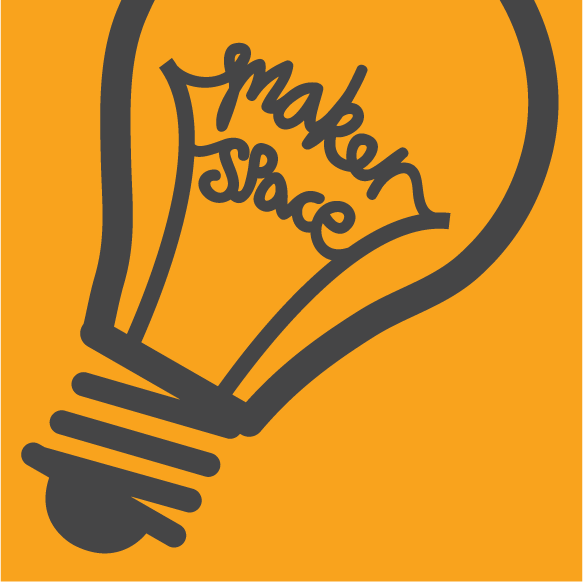
\includegraphics[scale=.1]{images/makerspace_logo.png}\\[1cm] % Include a department/university logo - this will require the graphicx package

\textsc{\Large Bachelor thesis}\\[0.5cm]
\textsc{\large BO19-G03}\\[0.5cm] % Minor heading such as course title

\HRule \\[0.4cm]
{ \huge \bfseries MakerSpace Management System}\\%[0.4cm] % Title of your document
\HRule \\[1.5cm]
 
\begin{minipage}{0.8\textwidth}
\begin{flushleft} \large
\emph{Authors:}\\
Andreas \textsc{Harnes},\\
Celina Marie \textsc{Kristiansen},\\
Magnus \textsc{Klerck},\\
Morten Offerdal \textsc{Kvigne}\\% Your name
\end{flushleft}

\end{minipage}\\[2cm]

% If you don't want a supervisor, uncomment the two lines below and remove the section above
%\Large \emph{Author:}\\
%John \textsc{Smith}\\[3cm] % Your name

%----------------------------------------------------------------------------------------
%	DATE SECTION
%----------------------------------------------------------------------------------------

{\large \today}\\[2cm] % Date, change the \today to a set date if you want to be precise

\vfill % Fill the rest of the page with whitespace

\end{titlepage}

\makepresentationpage
\addcontentsline{toc}{chapter}{Bachelor thesis}

\pagenumbering{roman}

\chapter*{Preface}
\addcontentsline{toc}{chapter}{Preface}

\chapter*{Summary}
\addcontentsline{toc}{chapter}{Summary}

\chapter*{Thanks to}
\addcontentsline{toc}{chapter}{Thanks to}

\newpage

\tableofcontents

\newpage

\addcontentsline{toc}{chapter}{Figures}
\listoffigures
\newpage

\addcontentsline{toc}{chapter}{Tables}
\listoftables
\newpage

\chapter*{Code list}
\addcontentsline{toc}{chapter}{Code list}

\newpage

\pagenumbering{arabic}

\chapter{Introduction}

\section{Project group}
The bachelor group consists of the following four IT students:
\begin{itemize}
    \item Andreas Harnes. 
    Computer Science student with interests in networking and programming.
    \item Celina Marie Kristiansen.
    Computer Science student with experience in databases and big data.
    She has previously been deployed at Logiq where she used Databricks to process data.
    \item Magnus Klerck.
    Information systems student with background as a computer electrician where he worked with IT maintenance and hardware repair.
    He also has an interest in cybersecurity.
    \item Morten Offerdal Kvigne.
    Computer Science student with interests in programming and data security.
\end{itemize}
Celina M. Kristiansen, Magnus Klerck and Morten Offerdal Kvigne have previously been working on projects together.
The three had effective collaborations in their former projects which is reflected in the results they produced.
Due to the effective collaboration the three of them decided to form this bachelor group.

Magnus and Morten had both previously worked with Andreas Harnes and they both believed him to be knowledgeable and as such he was brought in.

\section{Assignment provider}
MakerSpace is a workspace at Østfold University College in Halden. 
The workspace acts as a playground for students and employees who like to use technology to create something \cite{what-is-makerspace}.
MakerSpace is operated by Michael Andersen Lundsveen and 4 student assistants but all students and employees at Østfold University College have access to the facility 24 hours, 7 days a week
\cite{what-is-makerspace}.
Østfold University College describes the drive behind MakerSpace as:

\begin{displayquote}
The purpose of Makerspace is to offer students a physical space and an engaging environment with the aim to learn something new by encouraging curiosity and eagerness \cite{what-is-makerspace}.
\end{displayquote}
In addition MakerSpace also acts as an area for lectures, courses and experiments.
They also hold basic programming courses for children during the summer.

MakerSpace is equipped with various equipment related to several fields.
Some of the equipment MakerSpace offers is 3D printers, which can be used to print out different figures and shapes in plastic from a 3D model. Soldering irons for making circuits and soldering components, computers with VR headsets, lego robots and remote controlled drones as shown in figure \ref{fig:makerspace}. MakerSpace also has different tools like screwdrivers, workbenches, pliers, RJ45 crimpers to mention some.

Lastly MakerSpace allows students and employees at Østfold University College to borrow equipment.
Students and employees have to note down their name, their contact information and the item(s) they are lending in a book used to keep track of all borrowed equipment whenever they are borrowing equipment.

MakerSpace responsible Michael Andersen Lundsveen is the assignment provider for the project. 
Michael is the leader and principal engineer for MakerSpace Halden.
He oversees day to day operations and he ensures all equipment is in good condition.
Additionally he is responsible for the repairment or the purchase of new equipment should equipment be damaged or destroyed.
Michael also arranges courses for the MakerSpace employees allowing them to learn how to utilize new equipment, he arranges summer workshops for children during the summer vacations and he sponsors certain arrangements and events at Halden University College.

\begin{figure}
    \centering
    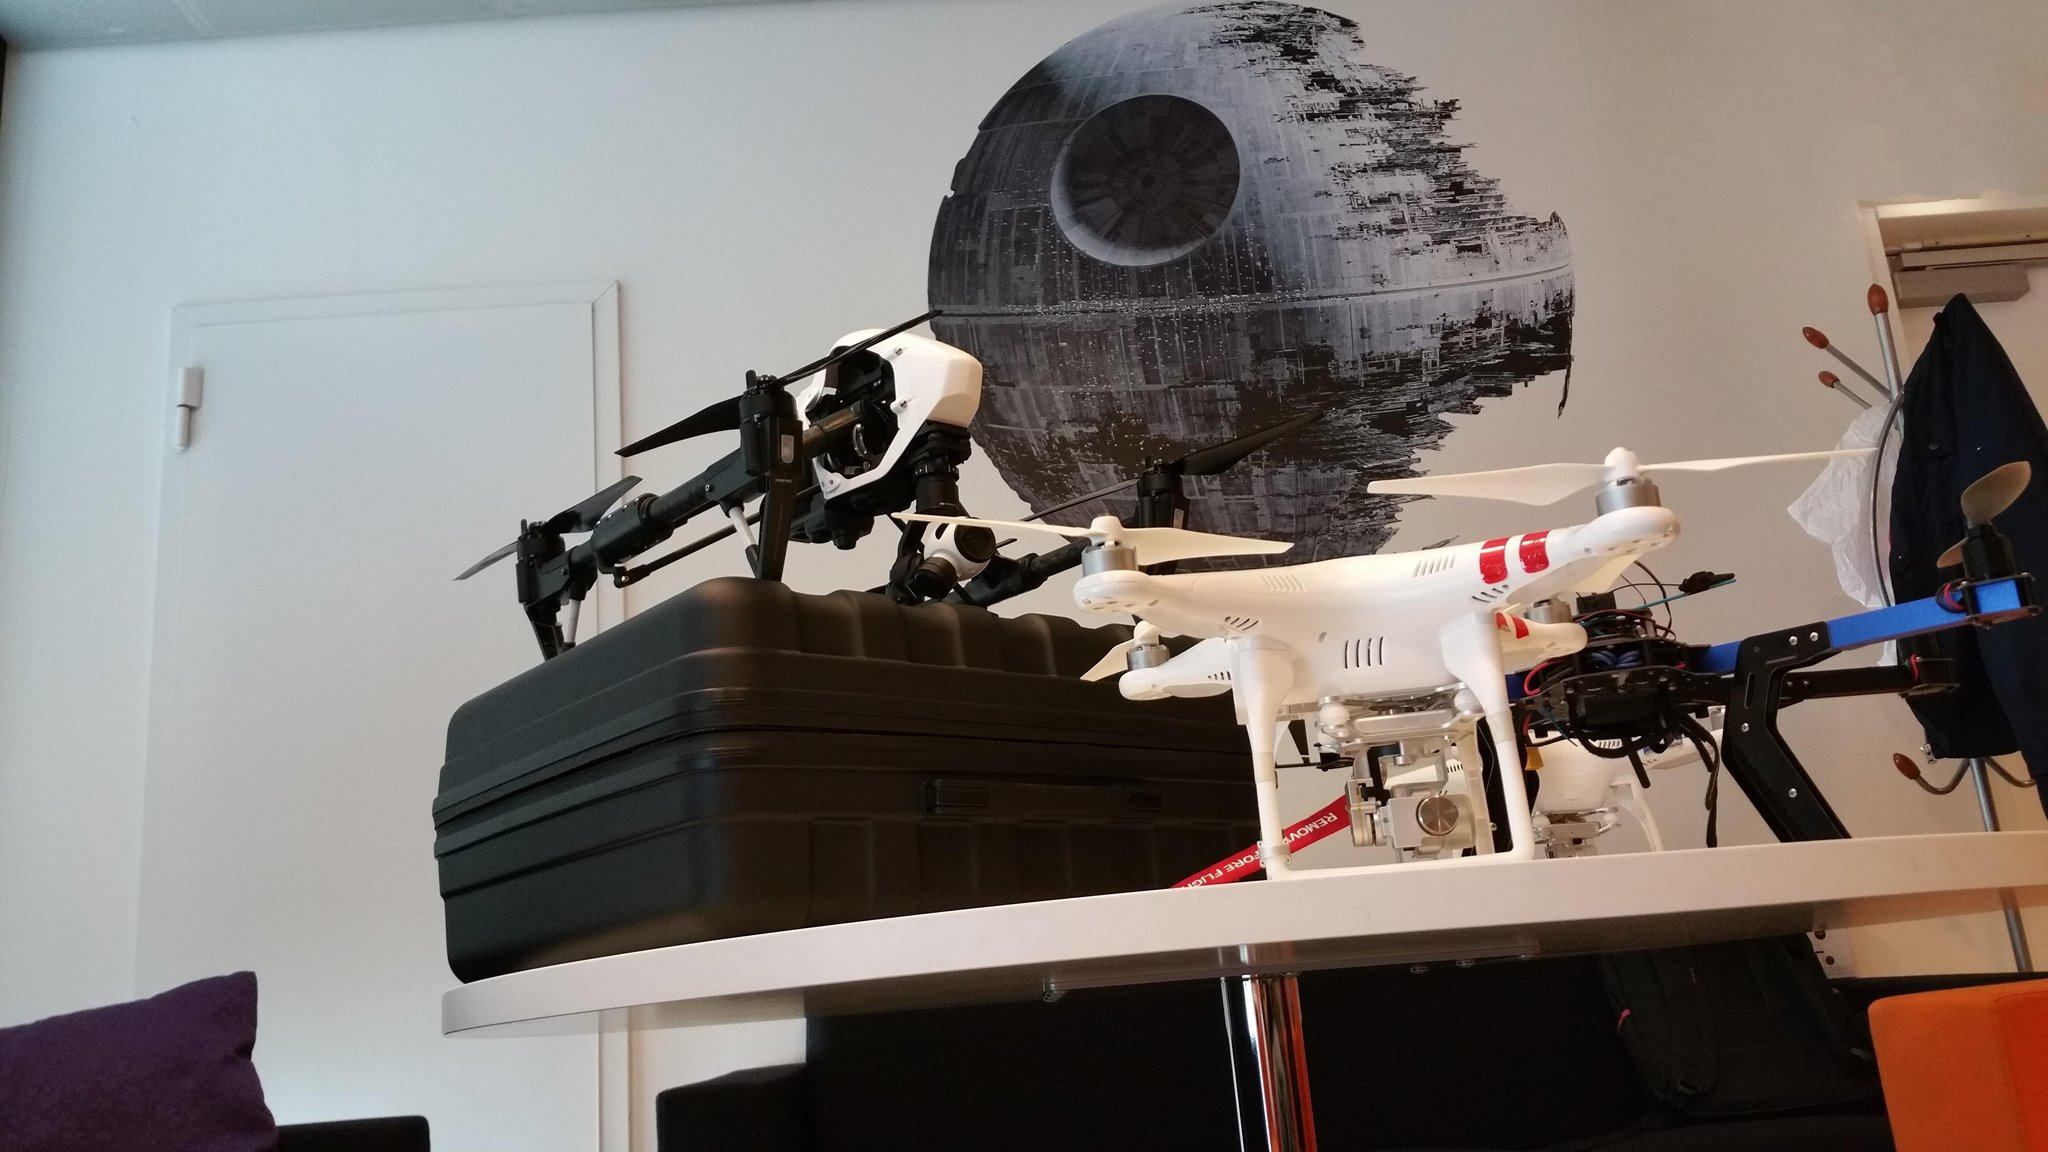
\includegraphics[width=115mm,scale=1]{images/makerspace.png}
    \caption{Remote controlled drone}
    \label{fig:makerspace}
\end{figure}

\section{The mission}
The background for the project is that MakerSpace currently does not have an overview of what equipment they have, whether said equipment is available and where said equipment is stored.
This is problematic for the employees at MakerSpace as they have no way of knowing whether equipment is missing or the equipment is damaged.
Even if an employee is made aware of missing or damaged equipment the employee currently has no way of notifying the other employees and as such the employee will have to manually contact the other employees in order to notify them which is hassling.

This is also problematic for the users of MakerSpace.
The users have to search through MakerSpace in its entirety in order to find a given piece of equipment.
They have no way of knowing whether the piece of equipment is damaged until they find it.
They also have no way of knowing whether MakerSpace does not offer said piece of equipment or whether another user is currently borrowing it should they not find it.

Lastly the book used when borrowing equipment also proves problematic.
Anyone can inspect the contents of the book and as such the book does not respect the privacy of the users.
This is especially concerning should the book be stolen.
Additionally the book can disappear.
Finally the book is not protected in the event of a fire.

In order to solve the issues outlined above the group intends to develop two modules.
The employees and users will interact with the modules using web pages.
The following two modules will be developed:
\begin{itemize}
    \item An inventory module allowing employees and users to view the equipment MakerSpace offers, the equipment's condition, where the equipment is stored and weather the equipment is available.
    The module will also allow employees to add, modify and delete equipment from the module.
    \item A lending module allowing employees and users to borrow equipment.
    When returning equipment the module also allows the employee or the user to report any damage that occurred whilst the equipment was being borrowed.
\end{itemize}

The modules will be extendable.
This allows future features to be incorporated into the modules without difficulties for future developers.

%What MakerSpace wants is a system that gives Michael and student assistants access to an overview of all the equipment and tools available in MakerSpace. This system must be modular so that it can be further developed later, and in addition to this a inventory system. They also want a lending module that makes it easier to register the lending of equipment and tools.

%What the group is planning to develop is a modular inventory system and a lending module by adopting technology that is in use today.

%\todo{TODO Alt under flyttes til metode}
%\textbf{Investigation:} The group have talked about some technology they could potentially use. Some of the technology the group have been thinking about is: Vue.js, Node.js and MongoDB. The group will do a investigation for each of those and find out if they fit the project or not. The group will also try and find other technologies that can be more applicable for the project.

%\textbf{Development:} The group will create a website that will offer a lending system of equipment that exists at MakerSpace and also make sure that the system can be further developed later on.

%In the development of the system, the group have made some bullet-points as an overview for the project. These are:
%\begin{enumerate}
%  \item Make the website that will be used for the system and make sure it follow the criteria for universal design.
%  \item Design a structure for the inventory storage.
%  \item Make a module for lending.
%  \item User test the system to find bugs.
%\end{enumerate}

\section{Purposes, delivery and method}
\subsection{Purposes}
%There are two reasons for the project.
%The first is to provide an overview of the equipment available at MakerSpace to the employees and users of MakerSpace.
%This is beneficial as the employees and users now no longer need to search through MakerSpace in its entirety to see if MakerSpace offers the equipment they seek.

%The second reason is to digitize the lending system MakerSpace currently has in place.
%This is beneficial because it is privacy respecting as only those with the necessary permissions can view the records of equipment currently being borrowed. 
%Additionally should equipment not be returned MakerSpace will know who is responsible.
%Lastly the records of borrowed equipment can be place on a backup - meaning the records of borrowed equipment are not lost in case of theft or in case of a fire.

\textbf{Main goal:} Make an inventory module which provides an overview of the equipment available at MakerSpace.

\textbf{Sub goal 1:} Make a lending module which digitizes the current lending system used at MakerSpace.

%The purposes with this project is to digitize the current lending system. This will make it easier to not only see what equipment that is available for lending but also what equipment that needs to be order more of. This is divided into a main goal and some sub-goal's.

%\textbf{Main goal:} Digitize current lending system and write the report.

%\textbf{Sub-goal 1:} Make a inventory structure with a lending module

%\textbf{Sub-goal 2:} Make sure that the website (e.g front-end, UI,UX) follow the criteria for universal design.

\subsection{Delivery}

Below are the deliveries the group will deliver during the project.

\begin{tabu} to 1.2\textwidth { | X[l] | X[c] | }
    \hline
    \textbf{Date} & \textbf{Delivery} \\
    \hline
    January 18 ,2019 & Pilot report \\
    \hline
    March 08, 2019 & First version of main document \\
    \hline
    April 23, 2019 & Second version of main document \\
    \hline
    April 26, 2019 & Product \\
    \hline
    May 16, 2019 & Finished version of main document \\
    \hline
    May 27, 2019 & Project poster \\
    \hline
   June 03, 2019 - June 05, 2019 & Presentation of the project \\
    \hline
\end{tabu}
    
\subsection{Method}
The group has decided to use an agile model for the software development process.
The project is small in scale and is not tightly integrated with any other system.
This means the comprehensive documentation a waterfall model requires is not needed.
Additionally this means informal communications between group members work well as the group is co-located.
The agile model does however require a higher presence of the assignment provider as he plays an integral part in which components the group are to prioritize.

The assignment provider is involved and accessible throughout the project development.
This allows for incremental development of the requirements set out by the assignment provider which means contract negotiations are not necessary.
Consequently the group can more easily adapt to changes in requirements as the documentation remains largely unaffected by the respective changes.
This is the driving factor behind the agile model:
\begin{displayquote}
Agile is the ability to create and respond to change.
It is a way of dealing with, and ultimately succeeding in, an uncertain and turbulent environment \cite{what-is-agile}.
\end{displayquote}
This is also one of the factors which separates the agile model approach to that of other software development models:

\begin{displayquote}
One thing that separates Agile from other approaches to software development is the focus on the people doing the work and how they work together.
Solutions evolve through collaboration between self-organizing cross-functional teams utilizing the appropriate practices for their context \cite{what-is-agile-software-development}.
\end{displayquote}
With everything taken into consideration the group believes an agile model is more suited for this project than that of a waterfall model.

The group believes the best way to organize the project is using the agile framework Scrum.
Scrum is a framework that is best suited for teams with a size of seven or less \cite{software-engineering-scrum-size} which makes the framework ideal for the group as the group consists of four members.
The assignment provider has set forth the features he would like to see in the system and these features make up the product backlog.
Given the fact that the assignment provider is so involved and accessible it seems fitting that he is involved in deciding which functionality is to be prioritized which Scrum allows him to do as a product owner.
The group believes the flexible approach an agile model used through Scrum provides the best foundation for the successful completion of the project.

%SCRUM (source: https://www.mountaingoatsoftware.com/agile/scrum) will be used as a framework to manage the project and the software development. SCRUM is a derivative of the Agile methodology, but we will use Agile (source:https://www.agilealliance.org) as the methodology when developing software for the project. The Agile method will be used so the group can adjust and adapt to changes in the development as the project goes along. By scaling this to the scope of the group and the project, Agile will fit the development of the project well. 

 When working on the report and documentation for the project it will follow qualitative research methods for gathering information and comparing/analyzing data. Qualitative research method is a scientific method of observation to gather non-numerical data. The aim of a qualitative research project may vary with the disciplinary background, like a mechanical engineer seeking in-depth understanding of a combustion engine for example.
 
 Qualitative methods are best for researching many of the why and how questions of something \cite{Qualitative-Research}. Qualitative research is widely used by political science, social work, and education researchers and only produce an explanation for the particular case that is studied. All the qualitative research done for this project will be focused on how we will do something and why that is the best way to do it. Like why did the group choose a certain program over another and how we are going to use said program. The reason for this is that the project does not need any quantitative data for the documentation of the project, one exception that might occur is in the testing phase. In the testing phase the project group will ask for a number of students and/or employees to test the developed system and it's ease of use i.g: UI, UE and possible bugs. The data collected from testing could be used to statistically to show that the UI and UX is good for all potential users. No matter how experienced the users are with IT or how many times the users have used the system.

\section{Report structure}

\textbf{Chapter 1, Introduction:}
Gives background information about the project as well as a brief summary of the methodology used.

\textbf{Chapter 2, Analysis:}
Provides a thorough description of the assignment based on the requirements set by the assignment provider in addition to explaining what the selected technologies are and why they are suitable for the project.

\textbf{Chapter 3, Design and planning:}
Explains how the components of the application are designed and how these components are intended to connect to form the final application.

\textbf{Chapter 4, Implementation:}
Describes how the application was built and which tools were used in doing so in addition to a description of the application itself.

\textbf{Chapter 5, Testing and Evaluation:}
Explains how the components of the application were tested - which components were tested, how were they tested and who tested them.
The chapter also provides the feedback received and whether the application passed the acceptance tests.

\textbf{Chapter 6, Discussion:}
Describes the project process - what went well, what did not and what could have been done differently.
The chapter also outlines what the group has learned during the project.

\textbf{Chapter 7, Conclusion:}
Presents the results and outlines the continuation of the project.


\chapter{Analysis}
\todo{Endre til at å si at vi har søkt, og michael var enig i valget}
This chapter provides the background knowledge required to understand the thought process behind the selected technologies.
The group have been advising the assignment provider as to suitable technologies for the project but the assignment provider has been the one selecting them.
The chapter first inspects the database technologies that are suitable for the assignment.
Afterwards the chapter examines the selected frontend technology before analyzing the technology stack used for the backend development.
Lastly the chapter provides insight as to why the methodology selected is the most suitable for the project.

\section{Analysis of different MakerSpaces}
The project group has decided to conduct interviews with different MakerSpace branches in Norway. The reason for choosing interviews is to be able to decide what information we want to get out of the interviewees. The project group will make a set of predetermined questions about how MakerSpace operates and what kind of systems and technologies they have. While conducting the interviews the project group also wants to arrange the interview at the respective MakerSpace, where the project group could get a tour of the MakerSpace and take a look at the systems they have and how they are used. This will be used to get more hands-on knowledge for the project, to be able to make a better system. The interviewee will also be more comfortable in a known environment during the interview.

\subsection{MakerSpace Inspiria}

This section is based on an interview the group conducted, as such the necessary sources are added as an attachment. The source is a voice recording of the interview transcribed. See page::::::::::::: %lage attachement/appendix side for vedlegg?%  

The first MakerSpace that was interviewed was MakerSpace Inspiria, located in Sarpsborg. It is part of Inspiria Science Centre \cite{Inspiria-SC}, a building full of science for people to enjoy and test out. It is mainly targeted for kids, but the MakerSpace is open for everyone when the centre is open. MakerSpace Inspiria is very much alike MakerSpace Halden. It's closely resembles each other and has a lot of the same equipment; 3D printers, laser cutters, soldering irons etc. 
And it is here the group conducted its first interview, at MakerSpace Inspiria. The interviewee answered all the questions best possible and the group got a lot of interesting information. There was no system in place for keeping tabs on the inventory, digital or other. The employees were the ones that kept control over the inventory personally, the employees shared responsibility of overseeing the inventory and ordering new parts and equipment when needed. But admitted to not having full control over everything. Components and tools are being kept in lockers and has a box i.e where similar tools or components are grouped and put together. There is however no special categorizing of the equipment, but everything has a predetermined place. 

As far as lending out equipment, MakerSpace Inspiria has no system in place for it and they do not lend equipment out. Exceptions could be made, depending on the person asking to loan something or the equipment in question. If an exception is made, the employee that loans something out is responsible for the item and its condition. If something is broken or gets broken, MakerSpace Inspiria has a system for reporting broken or faulty equipment. This system is used for the entire building (Inspiria Science Center). The employees report on the specific equipment that is broken and it is filed for review. The review consist of looking at the budget and the broken equipment to see if it is possible to order a replacement or if it is to expensive at the moment. This depends on what kind of equipment is broken. If it is an expensive 3D printer there might not be enough money in the budget to buy a new one e.g However if it is something smaller and not very expensive the employees doesn't report it broken and just orders a new one. 

When asked if a digital system for inventory keeping was something MakerSpace Inspiria could potentially want, the interviewee positively agreed. The interviewee already had an idea for a potential digital system. A simple bar-code and a scanner, zero thinking. Everything has its own ID and it gets scanned into a system. Everything about it has to be simple and have as few button presses as possible. This was from the interviewees own experience with people and IT, or more about people who doesn't know a lot about IT and would be using mentioned system. Other than that the interviewee didn't have any specific ideas on how the system should work or look. But the project group got some very nice ideas and pointers for the User Interface (UI) and User Experience (UX). Keep it nice and simple, not very complicated which is something the project group had already thought of. A bar-code was discussed early on in the project as a possible solution for both lending out equipment and inventory keeping. 

\subsection{Conclusion of the interview and questionnaire}

After an interview and getting 20 questionnaire responses from different MakerSpace's. The group has read through the responses and analyzed them. However, since all the answers are anonymous the group doesn't know which MakerSpace's that responded.   

The equipment each respondent have was varied, everything from digital tools and equipment and more heavy tools like CNC machines. Here is an overview of most of the equipment MakerSpace's in Norway have.

Heavy machinery (metalwokring tools)

Hand tools

Woodworking tools

Electronic tools

Electronic components

Acids

The amount of stuuf ranged from 1-22... 45 tons of equipment. skrive om mengde utstyr og alt som ikke apsset inn i listen.

Ut ifra spørreskjema så skriver vi hva vi fikk ut av det og hva vi lærte av det. Vi har ikke sendt ut spørreskjema enda så denne delen er av den grunn ikke fylt ut.

\todo{Why only looking at the two most popular? Why not others?}
\section{Database technology selection}
The two most popular database systems today are the SQL- and NoSQL-based database systems \cite{stackoverflow-db-statistics}.
The distinction between SQL and NoSQL database systems have become increasingly blurred \cite{sql-vs-nosql}, but there are still key differences between the two which makes them worth analyzing in order to find the most suitable database system for this project.

\iffalse
\subsection{CAP theorem}
The CAP theorem is a theorem within distributed database systems \cite{sql-schema}.
The theorem states that only two out of the following conditions can hold at any time:
\begin{itemize}
    \item Availability.
    This condition states that every request receives a (non-error) response.
    This means the data requested may not necessarily be up-to-date as the node may not have the up-to-date data \cite{sql-schema}.
    \item Consistency.
    This condition states that all nodes have access to the same data.
    This means whenever an attempt to extract data from the database is made the database will either provide up-to-date data or failure \cite{sql-schema}.
    \item Partitioning tolerance.
    This condition states that the database system will continue to operate despite any number of messages between the nodes being delayed or dropped by the network.
    This means the database system can operate normally while sustaining any number of network failures so long as not every node is experiencing failure \cite{sql-schema}.
\end{itemize}

A database is said to support AC when availability and consistency are selected, its said to support AP when availability and partitioning tolerance are selected and its said to support CP when consistency and partitioning tolerance are selected.
\fi

\subsection{SQL} 
SQL(Structured Query Language) is a database language for data management\cite{sql-goal} of a RDBMS(relational database management system) \cite{sql-is-a-rdbms} based on the relational data model proposed by Edgar Frank Todd \cite{rdbms}.
The relational data model logically structures all relations(tables) and each relation is provided a name and is built up of named attributes - columns of data \cite{sql-is-a-rdbms}.
The rows of a table are known as tuples \cite{sql-is-a-rdbms} and, provided the table is normalized for the first normal form or higher, they contain one value per attribute \cite{sql-1nf}.
Figure \ref{fig:relational-db-visualised} illustrates the relational model graphically.

\begin{figure}
    \centering
    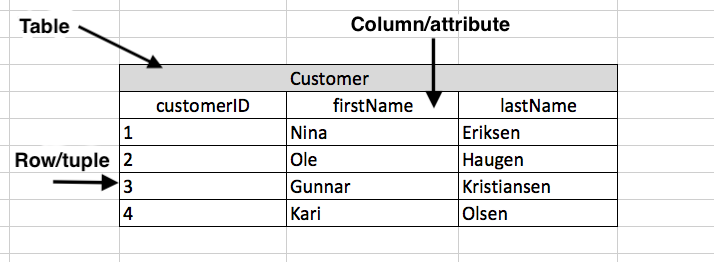
\includegraphics[width=115mm,scale=1]{figures/relational-db-visualised.png}
    \caption{Table named "Customer" containing three attributes and four tuples}
    \label{fig:relational-db-visualised}
\end{figure}

SQL offers a data definition language(DDL) \cite{sql-components}.
The DDL defines the database schema - that is the structure, meaning which attributes the tables consists of, and which tables the database consists of.
It is impossible to add data to the database until a schema has been defined.
The DDL also describes any relational integrities the tables of the database, or the columns of table, may have \cite{sql-constraints}.
In figure \ref{fig:relational-db-relation} a given customer may have several orders but a given order may have one and only one customer associated with it; this is an example of a one-to-many relationship.
In addition to a one-to-many relationship an attribute or table may also have a one-to-one or a many-to-many relationship \cite{sql-relationships}.
Lastly the DDL also defines any security constraints the database may have - such as which users have permissions to read, update or delete the contents of a given table \cite{sql-ddl}.

\begin{figure}
    \centering
    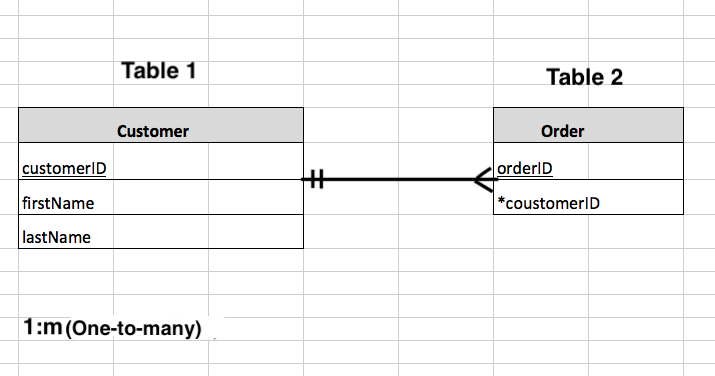
\includegraphics[width=115mm,scale=1]{figures/relational-db-relation.png}
    \caption{One-to-many relation between "Customer" and "Order"}
    \label{fig:relational-db-relation}
\end{figure}

SQL also offers a data manipulation language(DML) \cite{sql-components}.
The DML allows for the insertion of, retrieval of, update of, and deletion of data \cite{sql-dml-options}.
Whenever a tuple is added, updated or removed the tuple must conform to the restraints set by the DDL.
The attempted action will be aborted should there be discrepancies between the constraint of the table or column and the data.
This ensures that the data in the table is accurate and reliable \cite{sql-constraints}.

In addition SQL:
\begin{itemize}
    \item Provides an organized structure as data is defined once, and items referencing the data does so using foreign keys \cite{upwork-sql-adv}.
    \item Reduces data redundancy due to the organized structure \cite{upwork-sql-adv}.
    \item Allows JOIN operations \cite{upwork-sql-adv}.
    The operation allows two or more tables to be combined based on some shared attribute between them.
    The JOIN operation provides the ability to fetch specific data across tables that otherwise would prove cumbersome \cite{sql-joins}.
    \item Provides support for transactions.
    Transactions are essential in databases which require reliable data as they provide a framework for an all-or-nothing approach.
    This means the sequence of involved operations have to succeed in its entirety.
    The database will perform a rollback and raise an error should one of the operations fail \cite{sql-transactions}.
\end{itemize}

\subsection{NoSQL}
A NoSQL(Not only SQL) database provides data storage and data retrieval capabilities that is not modeled using a conventional RDBMS \cite{nosql-not-rdbms}.
Schema-less models are used instead of the traditional RDBMSs.
The most popular models include:
\begin{itemize}
    \item Key-value stores.
    Every item in the database is stored as an attribute name with a corresponding value \cite{mongodb-explains-nosql}.
    The key and value can be anything, and the key acts as a unique identifier for the value \cite{nosql-key-value}.
    \item Document databases.
    Document databases are an extension to key-value stores.
    Documents are structures which can contain many different key-pairs, and documents can even contain other documents.
    The documents can store data in different format, such as XML or JSON.
    Document databases are intended to store semi-sorted data \cite{nosql-document-sort}.
    \item Wide-column stores.
    The data in the database is stored in columns rather than the typical SQL rows.
    A given row can therefore have columns that other rows does not have.
    A wide-column store can be considered a two-dimensional key-value store \cite{infoworld-sql-vs-nosql}.
    \item Graph stores.
    The data in the database is represented as a graph.
    Their intended use is to traverse and navigate relationships.
    These databases use nodes to represent items in the database, and an edge between two nodes represents a relationship between the two items \cite{nosql-graph}.
\end{itemize}

NoSQL is advantageous because it:
\begin{itemize}
    \item Allows for semi-structured or unstructured data in the database.
    This flexible design allows the database to handle changes in structure more easily, and also allows the database to scale with ease \cite{mongodb-adv-nosql}.
    \item Allows for data to be inserted without a schema \cite{omkarsoft-adv-nosql}.
    This is beneficial should data be expected to change during the development of the project.
    \item Scales horizontally rather than vertically \cite{mongodb-adv-nosql}.
    Scaling horizontally allows partitions of data to be scatted across several pieces of hardware in order to store the data in the database.
    By contrast, scaling vertically means replacing already-existing hardware with more powerful hardware \cite{technopedia-nosql-scale}.
\end{itemize}

\subsection{Why SQL is the selected database system}
The assignment provider believes a SQL database system is more suited for the project than that of a NoSQL database system.
The equipment provided at MakerSpace is limited in quantity - as such the data to be stored in the database is also small in scale.
Due to the limited data the schema is simple to define, and as the requirements for the project are unlikely to change at a structural level the flexibility a NoSQL schema provides is not necessary.
The database is also likely to be stored in a limited number of locations and as such the distributed scaling capabilities a NoSQL database system offers is not particularly beneficial.
Overall the benefits provided by a NoSQL database system are not well suited for the project nor the scope of it which makes the SQL database system the preferable choice due to its organized structure, its relational properties and its support for JOIN operations.

\subsection{MariaDB as software}
MariaDB is the assignment providers database management system of choice.
MariaDB is one of the most popular\cite{mariadb-foundation-about} open source relational database management systems in the world \cite{mariadb-about}.
It is a fork of the also popular relational database management system MySQL\cite{mysql-about}.
MariaDB is made by the original developers behind MySQL \cite{mariadb-foundation-about} and it has a large list of sponsors providing financial support including Microsoft and IBM \cite{mariadb-sponsors}.
MariaDB is based on the SQL database system \cite{mariadb-about-searchdatamanagement}.

MariaDB has several notable features.
It is able to handle small and large data alike making it highly scalable, and it allows for rapid access to the data.
MariaDB releases stable releases, and each new release brings speed and stability improvements in addition to new features.
Additionally it places a high value of security - all data is encrypted by default and whenever critical security issues arise a new release is prepared \cite{mariadb-about}.
Lastly MariaDB offers a Node.js connector allowing applications developed on Node.js to connect to MariaDB \cite{mariadb-node-connector}.

\todo{Ikkje bruk several - ver konkret.}
\section{Frontend technology selection} 
The assignment provider wanted a full JavaScript technology stack and as such there were several technologies that could have been chosen for the frontend development.
There are several JavaScript frontend frameworks and libraries freely available and as such this was not a limitation.

The assignment provider ended up choosing Vue.js because of three major factors; the size of the framework, live updating in the browser and the low learning curve it has. Vue.js is comparably smaller than many of the other big JavaScript frameworks. It is roughly 58.8 kB in size. Since the framework is so small it will help with the loading speed of the web application \cite{vue-size}. 

The second major point for choosing Vue.js was the reactivity of Vue. With the reactivity of Vue.js you could update individual components based off of which data had been updated in the database. In Vue.js each component has getters and setters that enables Vue to track each component for when it's been accessed or modified. Each component also has a watcher instance that will be notified when that components setter is triggered. When this happens the watcher will notify Vue to run the component render function on that component again. With this feature there will be no need to update the whole site to show an update in the database \cite{vue-reactivity}. 

\begin{figure}
    \centering
    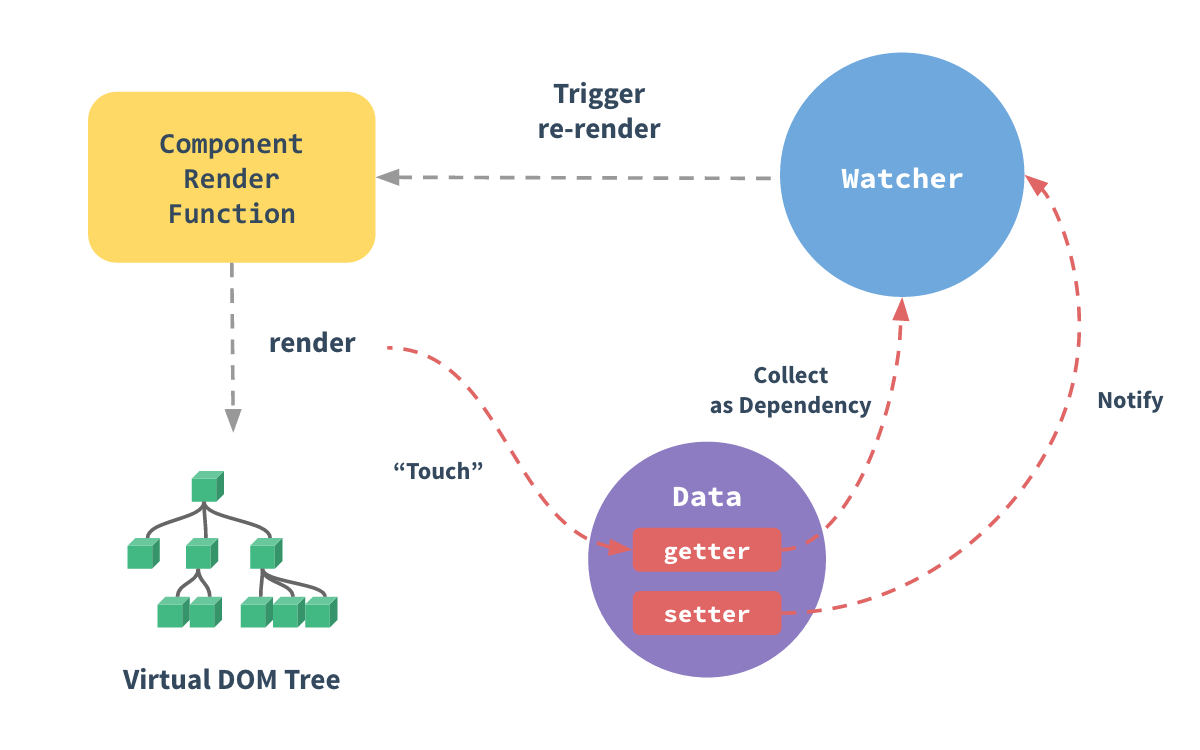
\includegraphics[width=115mm,scale=1]{figures/reactivity.png}
    \caption{Reactivity in Vue.js}
    \label{fig:vue_reactivity}
\end{figure}

The last major point for the group was the low learning curve of Vue.js. With this learning curve it means that the easier parts of Vue.js is easier to learn, but the more complicated components can be harder. This is perfect for the groups project since all the group members are new to Vue.js and can get faster into the programming.

\section{Backend technology selection}
\todo{en måte: alternativ valg +/- valget}
For the backend technology there are several technologies that could be used. The group had discussed what backend technology to use, and asked the assignment provider to choose. A full JavaScript technology stack was chosen and some of the major backend technologies have been ruled out. Such as Pythons Django, PHP or Javas Spring backend framework. 

JavaScript will be used for the backend, Node.js will be used as the server to create and handle the backend operations needed in the application. Node.js is a JavaScript run-time environment that can run JavaScript code outside of the browser using the V8 JavaScript engine. Node.js runs on a single thread and is able to do this because of the Event Loop. When a request gets sent to Node from the application it will be added to the event queue before being picked up by the Event Loop. The Event Loop will take these requests and send them to the system that Node runs on. Here each request will be sent to different threads and be completed. When the task in done a callback function in the request is activated and the feedback is sent directly back to the application. The reason this event loop is so efficient at handling requests is because it runs asynchronous. So when it receives a request and sends off a callback function for that request. It doesn't need to wait for that callback function to return something before it handles a new request \cite{Node-event-loop}.

\begin{figure}
    \centering
    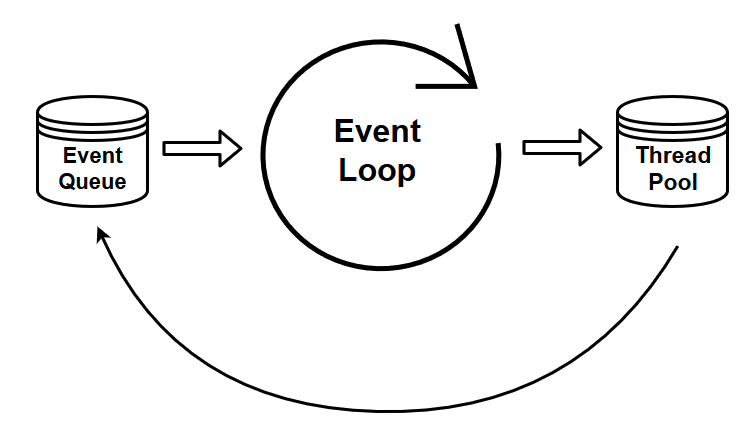
\includegraphics[width=115mm,scale=1]{figures/event_loop.png}
    \caption{Event loop in Node.js}
    \label{fig:Node_Event_Loop}
\end{figure}


\input{chapters/design-and-implementation}

\chapter{Evaluating and testing}
In this chapter it can be read about the evaluating and testing method that is been done for the project. For the first part it can be read about the heuristic evaluation where the focus has been looking for some design idea that can be implemented and where it has also provided the basis for a wireframe. For the second part it could be read about the usability test that has been done. With that it can be seen how well the user could use the system, what errors that emerge and how well the functionality works so fare. 

\section{Heuristic evaluation}
The purposes with this heuristic evaluation is that the group is going to look at a another website that share some of the similarity as the group think the system in development will have. For this evaluation the group alongside with the assignment provider has decided that they are going to look into finn.no website. The test itself will be performed by one of the group members and by the assignment provider.

FINN is a website where users can exchange and sell stuff that they have at home. The group think that by looking at FINN, it will give some ideas to how the inventory system will look like, categorizing things and what kind of layout the website will have. FINN have also been nominated for best interactive design,
and considered to have good universal design.\cite{finn_nominert}
That makes it a good choice to look into, since universal design is also something the group need to implement in the development of the system. 

As mentioned in the section about method, when doing a heuristic evaluation there needs to be some rules set in place. These rules needs to be followed throughout the evaluation. The rules should contain what things that will be look for when doing the evaluation. The heuristics that have been agreed to are:

\subsection{Heuristics}
\begin{enumerate}
  \item How are things categorized?
  \item How does search work?
  \item How many things can you see on a page before switching? 
  \item Can you create your own user?
  \item Is it easy to find contact information?
  \item How does navigation work?
  \item Can you store things you are interested in?
  \item What does the buy item contain?
 \end{enumerate}

%Legger til vedlegg av selve test dokumentet/resultater%

\subsection{Summary}


\section{Usability testing}
Since the group decided to use heuristic evaluation to try to look for some good ideas about design and how items have been 
categorized, the usability test will now be used to test the functionality for the system they are building. This to find out if the things the group has developed is working, or if there are bugs and perhaps some additional components that can be added.

The group will do this test on those who work on MakerSpace to see if they wish something was done different or if they feel something is missing to meet the needs for this system. The group will also find other students from other educations than Information Technology (IT), to see if those students can find different errors. Since this system is not only for the students that studies IT, but the whole school, it is important to test different students from different studies to make it fit everyone.

At this time the group already now that the system are facing some issues. Things like the user will not know the rules of how making a password and they will not know if the registration is done correctly, therefore the monitor of the test will give some help before going to next task. The monitor i suppose to be passive, but without any help it can be hard to test the actually functionality of this system. Other things is that items is at the moment before testing not displaying so it might be hard for the user to understand that they got right when looking for items.

Below you can read about how the group will conduct the usability test and how the result for the tests are.

\subsection{Test plan}
\textbf{Purpose:} The purpose of this test is to detect errors and test the functionality of the system.

\textbf{Problem statement:} The problem that will be tested will be if the participant can register a new user, alongside if the participant can log in with the user he/she created. Another thing that will be tested is if the participant can navigat back to the home page/item page. More details of the exact tasks are found in "Task list" bellow. 

\textbf{Test roles:} In this test it will be two different roles. One moderator and one observer. The moderator will be the one who heads the test. With that it means the moderator will read out the problems/task that the participant will be doing and also give out follow-up questions. The moderator role will be semi-open. That means the moderator will not help the participant with the test, but can can answer questions that the participant have, if there are some unclear things about the test task.

The observer role will be completely passive. The only thing the observer will do is to note down some data that is gonna be collected by this test. It can be a certain behavior that the participant have through the test, like wrong "click" or how long it takes for the participant to complete the test. Other behavior which can affect the test result will also be noted by the observer. Since it will be used a Thinking Aloud method, the observer will need to note down what the participant is thinking when doing the test. 

\textbf{User profile:} The user that will be tested is two persons that work at MakerSpace and the group will also find one other student on the school for example, a teacher student.

\textbf{Methodology:} 
The group has decided that they will divide the test in this four steps:
\begin{enumerate}
    \item \textbf{Background questionnaire:} This is where the moderator for the test collect background information about the participant before starting the test. This is going to be be gender, age and what education they take, or whether it is a student or a teacher. The moderator also make sure that the anonymity agreement will be signed before starting \textit{(see appendix "Use test template")}.
    
    \item \textbf{Orientation:} The moderator will read and give out different problems/tasks that the participant will perform.
    
    \item \textbf{Performance test:} When the participant is preforming the test, then the observer will take notes of different things that has been agreed to collect.
    
    \item \textbf{Participant debriefing:} After the test is done, the moderator will ask some follow-up questions. This is to find out how the participant felt the test went or if they have anything else they want to add before finishing the test.
\end{enumerate}
\textbf{Task list:}
\begin{table}[h]


\begin{tabular}{lllll}
 \textbf{Nr.} & \textbf{Task} & \textbf{Claims} & \textbf{
Measure}  \\
\textbf{1.} & Create a new user &  Use drop down menu & Time, errors \\
\textbf{2.} & Log in with user & Use drop down menu & Time, errors  \\
\textbf{3.} & Get back to homepage & Use drop down menu & Time, errors 
\end{tabular}
\end{table}

\begin{table}[]
\begin{tabular}{ll}
\textbf{Nr.} & \textbf{Description} \\
\textbf{1.} & You want to make a new user on MakerSpace Management System, how will you do it? \\
\textbf{2.} & You will now log in with the user you created, how will you do it? \\
\textbf{3.} & You are now logged in and will look at equipment that MakerSpace have, how will you do it? 
\end{tabular}
\end{table} 

\textbf{Test environment and equipment requirements:} The test will be carried out in a group room at the school. That will make sure that the participant will not be disturbed while conducting the test, as that the group room is a quiet place.  

Equipment that is needed is a computer with the latest functioning version of the MakerSpace Management System. A few pens is needed and also a physical copy of the test tasks, one to the moderator and one for each of the observers and participant. A paper where the moderator collect background information, and a something the observer can takes notes on.

\textbf{Evaluating measure:} The main thing that will be tested or be collect is if the system work. The group will check if the participant is able to register a new user and log in with it. The observer will take notes of all the errors the participant do. For example if the participant can't find the log in site or don't understand how or what he/she is going to fill out. The time it takes for the participant to complete each task will also be measured.

\subsection{Summary}
The age of the participant was between 20-30 years. Two of the participant is studying IT and one studying teacher. For all of the participant the whole test went very fast. For each task all of them spent between one minute and 30 seconds to about 40 seconds to complete the task. 

On task one there was none of the participant that successfully could create a valid user. That was something that was expected, since the group had not added use feedback. Otherwise did none of the participant have any issue to find and fill out the information. Although none had any big issue finding registrar, they still think it was a bit silly to have the link in the drop down, instead of a menu link. The group will consider taking out both log in and registrar from drop down to make it even easier for the user to find it.

Task two went well for all of the participant, after the monitor help the participant to make a valid user before moving on to this task. None had any big issues, only as in registrar that they wish it was in the header menu instead of drop down. Another feedback was that one of the participant wish the system had a enter function, so it is possible to just hit enter when done filling out instead of clicking the actually log in button.

The last task went well too, but although all of the participant found back tho the right page, they was facing some confusion. This was also something that was expected since the was no real item displayed on that page jet. That made some participant to start clicking on other stuff on the page, as available button and so on. Some feedback was that someone tried to click on the logo, cause they thought that would take them back to front page, something it did not. 

On the question of how hard the participant think it was to complete each task, they think the first task was a bit tricky and confusing, but after getting a valid user they had no problem completing the two other tasks. Other feedback was as mentioned more visible menu and enter functionality. The group will take all the feedback into and make the system better. 



\chapter{Discussion}
 The content in discussion will be about the project groups own thoughts on the projects, and discussions around it.

\chapter{Conclusion}
Presents the results and outlines the continuation of the project.

\printbibliography

\end{document}
